\def\year{2020}\relax
%File: formatting-instruction.tex
\documentclass[letterpaper]{article} % DO NOT CHANGE THIS
\usepackage{aaai20}  % DO NOT CHANGE THIS
\usepackage{times}  % DO NOT CHANGE THIS
\usepackage{helvet} % DO NOT CHANGE THIS
\usepackage{courier}  % DO NOT CHANGE THIS
\usepackage[hyphens]{url}  % DO NOT CHANGE THIS
\usepackage{graphicx} % DO NOT CHANGE THIS
\usepackage{multirow}
\urlstyle{rm} % DO NOT CHANGE THIS
\def\UrlFont{\rm}  % DO NOT CHANGE THIS
\usepackage{graphicx}  % DO NOT CHANGE THIS
\frenchspacing  % DO NOT CHANGE THIS
\setlength{\pdfpagewidth}{8.5in}  % DO NOT CHANGE THIS
\setlength{\pdfpageheight}{11in}  % DO NOT CHANGE THIS
%\nocopyright
%PDF Info Is REQUIRED.
% For /Author, add all authors within the parentheses, separated by commas. No accents or commands.
% For /Title, add Title in Mixed Case. No accents or commands. Retain the parentheses.
 \pdfinfo{
/Title ( Outer Dictionary Network: An Efficient Network to Join Knowledge for Named Entity Recognition )
/Author (Junxiang Ge, Qi Zhang, Haizhou Zhao)
} %Leave this	
% /Title ()
% Put your actual complete title (no codes, scripts, shortcuts, or LaTeX commands) within the parentheses in mixed case
% Leave the space between \Title and the beginning parenthesis alone
% /Author ()
% Put your actual complete list of authors (no codes, scripts, shortcuts, or LaTeX commands) within the parentheses in mixed case. 
% Each author should be only by a comma. If the name contains accents, remove them. If there are any LaTeX commands, 
% remove them. 

% DISALLOWED PACKAGES
% \usepackage{authblk} -- This package is specifically forbidden
% \usepackage{balance} -- This package is specifically forbidden
% \usepackage{caption} -- This package is specifically forbidden
% \usepackage{color (if used in text)
% \usepackage{CJK} -- This package is specifically forbidden
% \usepackage{float} -- This package is specifically forbidden
% \usepackage{flushend} -- This package is specifically forbidden
% \usepackage{fontenc} -- This package is specifically forbidden
% \usepackage{fullpage} -- This package is specifically forbidden
% \usepackage{geometry} -- This package is specifically forbidden
% \usepackage{grffile} -- This package is specifically forbidden
% \usepackage{hyperref} -- This package is specifically forbidden
% \usepackage{navigator} -- This package is specifically forbidden
% (or any other package that embeds links such as navigator or hyperref)
% \indentfirst} -- This package is specifically forbidden
% \layout} -- This package is specifically forbidden
% \multicol} -- This package is specifically forbidden
% \nameref} -- This package is specifically forbidden
% \natbib} -- This package is specifically forbidden -- use the following workaround:
% \usepackage{savetrees} -- This package is specifically forbidden
% \usepackage{setspace} -- This package is specifically forbidden
% \usepackage{stfloats} -- This package is specifically forbidden
% \usepackage{tabu} -- This package is specifically forbidden
% \usepackage{titlesec} -- This package is specifically forbidden
% \usepackage{tocbibind} -- This package is specifically forbidden
% \usepackage{ulem} -- This package is specifically forbidden
% \usepackage{wrapfig} -- This package is specifically forbidden
% DISALLOWED COMMANDS
% \nocopyright -- Your paper will not be published if you use this command
% \addtolength -- This command may not be used
% \balance -- This command may not be used
% \baselinestretch -- Your paper will not be published if you use this command
% \clearpage -- No page breaks of any kind may be used for the final version of your paper
% \columnsep -- This command may not be used
% \newpage -- No page breaks of any kind may be used for the final version of your paper
% \pagebreak -- No page breaks of any kind may be used for the final version of your paperr
% \pagestyle -- This command may not be used
% \tiny -- This is not an acceptable font size.
% \vspace{- -- No negative value may be used in proximity of a caption, figure, table, section, subsection, subsubsection, or reference
% \vskip{- -- No negative value may be used to alter spacing above or below a caption, figure, table, section, subsection, subsubsection, or reference

\setcounter{secnumdepth}{0} %May be changed to 1 or 2 if section numbers are desired.

% The file aaai20.sty is the style file for AAAI Press 
% proceedings, working notes, and technical reports.
%
\setlength\titlebox{2.5in} % If your paper contains an overfull \vbox too high warning at the beginning of the document, use this
% command to correct it. You may not alter the value below 2.5 in
%\title{AAAI Press Formatting Instructions \\for Authors Using \LaTeX{} --- A Guide }
\title{ Outer Dictionary Network: An Efficient Network to Join Knowledge for Named Entity Recognition }
%Your title must be in mixed case, not sentence case. 
% That means all verbs (including short verbs like be, is, using,and go), 
% nouns, adverbs, adjectives should be capitalized, including both words in hyphenated terms, while
% articles, conjunctions, and prepositions are lower case unless they
% directly follow a colon or long dash
%\author{Written by AAAI Press Staff\textsuperscript{\rm 1}\thanks{Primarily Mike Hamilton of the Live Oak Press, LLC, with help from the AAAI Publications Committee}\\ \Large \textbf{AAAI Style Contributions by
%Pater Patel Schneider,} \\ \Large \textbf{Sunil Issar, J. Scott Penberthy, George Ferguson, Hans Guesgen}\\ % All authors must be in the same font size and format. Use \Large and \textbf to achieve this result when breaking a line
%\textsuperscript{\rm 1}Association for the Advancement of Artificial Intelligence\\ %If you have multiple authors and multiple affiliations
% use superscripts in text and roman font to identify them. For example, Sunil Issar,\textsuperscript{\rm 2} J. Scott Penberthy\textsuperscript{\rm 3} George Ferguson,\textsuperscript{\rm 4} Hans Guesgen\textsuperscript{\rm 5}. Note that the comma should be placed BEFORE the superscript for optimum readability
%2275 East Bayshore Road, Suite 160\\
%Palo Alto, California 94303\\
%publications20@aaai.org % email address must be in roman text type, not monospace or sans serif
%}
\author{Junxiang Ge, Qi Zhang, Haizhou Zhao\\ 
AI Research Department, Sogou Inc. \\
Beijing, China \\
\{gejunxiang, zhangqi215814, zhaohaizhou\}@sogou-inc.com}
 \begin{document}

\maketitle

\begin{abstract}
%AAAI creates proceedings, working notes, and technical reports directly from electronic source furnished by the authors. To ensure that all papers in the publication have a uniform appearance, authors must adhere to the following instructions. 
In many AI applications, we need to extract some specific types of message from user's query, which is the main content of Named Entity Recognition (NER) task. In recent years, dictionary, one kind of outer knowledge, is proved to be important in NER tasks, and applied more and more constantly. Howerver, most of the current networks use it as word embedding vector, which will bring out such problems: a) out of vocabulary (OOV) problem; b) we need to retrain model when the list of words in dictionary is greatly changed. In this paper, we propose a new conception, called Outer Dictionary Network (ODN), which means to join the outer knowledge of dictionary into Neural Networks (NN), without using the specific word or word embedding vector. We prove in our paper that, the two mentioned problem will be solved in this way. We then propose a new structure, called Tag Embedding LSTM (TE-LSTM) to implement the ODN. Experiment results show that our model acheive a great improvement on several tasks within which dictionary is heavily depended on, with comparison with current state-of-the-art methods. And the network will change its output along with the content variation of dictionary, without training the model again.
\end{abstract}

%\noindent Congratulations on having a paper selected for inclusion in an AAAI Press proceedings or technical report! This document details the requirements necessary to get your accepted paper published using PDF\LaTeX{}. If you are using Microsoft Word, instructions are provided in a different document. AAAI Press does not support any other formatting software. 
%
%The instructions herein are provided as a general guide for experienced \LaTeX{} users. If you do not know how to use \LaTeX{}, please obtain assistance locally. AAAI cannot provide you with support and the accompanying style files are \textbf{not} guaranteed to work. If the results you obtain are not in accordance with the specifications you received, you must correct your source file to achieve the correct result. 
%
%These instructions are generic. Consequently, they do not include specific dates, page charges, and so forth. Please consult your specific written conference instructions for details regarding your submission. Please review the entire document for specific instructions that might apply to your particular situation. All authors must comply with the following:
%
%\begin{itemize}
%\item You must use the 2020 AAAI Press \LaTeX{} style file and the aaai.bst bibliography style file, which are located in the 2020 AAAI Author Kit (aaai20.sty and aaai.bst).
%\item You must complete, sign, and return by the deadline the AAAI copyright form (unless directed by AAAI Press to use the AAAI Distribution License instead).
%\item You must read and format your paper source and PDF according to the formatting instructions for authors.
%\item You must submit your electronic files and abstract using our electronic submission form \textbf{on time.}
%\item You must pay any required page or formatting charges to AAAI Press so that they are received by the deadline.
%\item You must check your paper before submitting it, ensuring that it compiles without error, and complies with the guidelines found in the AAAI Author Kit.
%\end{itemize}

\section{Introduction}
Named Entity Recognition (NER) is a base task in Natural Language Processing (NLP) domain. Usually, we need to extract main information from users' sentences to help us understand their meanings, and then use the extracted information to do further process. For example, in weather domain, we may need to extract entities \textbf{date and position} to help us understand when and where the user is asked towards the weather; in music playing service, we may need to track entities \textbf{singer, song, style}  to suit user's command; for 	many commom use, we may need entities \textbf{person, location, organization} to understand a sentence.

To accomplish this task, many method has been explored.  Convolution Neural Network (CNN) is first used in Image Classification \cite{cnn}, and then also proved powerful in Text Classification \cite{kim}. Therefore, CNN is also useful in NER tasks, whether to capture character-level features \cite{char-fea1,mahovy,peter2017}, or to do word-level sequence labelling jobs \cite{santos,strubell}. To learn the correlation between words in sentence, Recurrent Neural Network (RNN) \cite{rnn} and Long Short-Term Memory (LSTM)  \cite{lstm} are proposed, and they achieve great success on machine translation and many other areas \cite{lstmbcp}. They are then used in NER tasks and achieve significant improvement. These structures can be combined together and used in different situations \cite{comb}.

Among these years, many works have made innovative attempts on constributing new NN structures. These models, like Transformer structure \cite{vaswani} and its derivative methods, like OpenAI GPT \cite{openai}, BERT \cite{bert}, XLNet \cite{xlnet}, focus on base layer of NN structure, usually the embedding input layer, to get better sentence understanding. The output of these models can then be directly fed it or fine-tuned to do NLP tasks \cite{bertslot}. Though will they make great improvement, it usually pays a long time to train these models. Through these works, we can conclude that, \textbf{The better and richer input knowledge there is, more efficient the model will be}. 

Among NER tasks, there exists a little difference between different languages. In Chinese or other hieroglyphics language, a character is also a single word; and Chinese word is ofter referred to a character phrase which has length longer than one. In English or other letter-based language, character means a single letter, and word is a composition of letters; that is to say, English word is composed by characters, for which character level CNN can help improve NER tasks \cite{huang15,char-fea1,mahovy,peter2017,peter2018,comb}; but that can not be used in Chinese NER tasks, which is hieroglyphics, no letter is there in a word. What we call character embedding in Chinese NER tasks correspond to word embedding in English jobs; and the so-called word embedding in Chinese NER jobs is likened to word phrase embedding in English. For this reason, Chinese NER tasks is usually done by word baseline or character baseline structure, which has the different meaning with English NER tasks. Among Word baseline structures, we may use word segmentor to split sentence into word tokens, and then use word embedding to turn these token into vectors \cite{peng15,peng16}; while character structures simply treat each sentence as a sequence of Chinese characters, and then using corresponding character embedding to do NLP tasks \cite{lattice,lrcnn}. Furthermore, it seems useful when using word embedding within character baseline structure, or the oppisite, cause it can enrich the input knowledge. Recently, more and more Chinese datasets \cite{msra,peng15,lattice} have been released to further research for Chinese NER research.  

On the higher layer, most of the state-of-the-art NER methods use Conditional Random Fields (CRF) \cite{crf} to decode the sequence labelling result and compute loss. CRF can work even without any NN cells. Hand-crafted features already achieve high performance \cite{stner,CRFsuite} on many jobs. 

Though with these powerful networks, word backgound knowledge, usually dictionary (same meaning to lexicon and gazette), is still necessary to do NER jobs in some situations. For example, in music playing service, ``You raise me up'' would be treated more likely as a chat intention rather than a song intention, unless the model is given that knowledge (see in Figure \ref{fig_gazzete}). Most of the state-of-the-art methods use word embedding \cite{glove,fasttext} to complete these tasks. But it then gives two problems: 

\begin{itemize}
\item Out of vocabulary (OOV) problem. To our knowledge, word embedding will always lead to this problem. Furthermore, it is hard and burdersome to make embedding vector for every word in dictionary. As for entity \textbf{song} in music playing service, word embedding size will be too large; and sometimes will the length of song be too long to make word vector. 
\item Retraining problem. When the content of dictionary changes abundantly, the trained model would have poor performance doing the same job. Still use the entity \textbf{song} as an example, the dictionary would be changed monthly or even daily, which forces us to retrain the model synchronously. 
\end{itemize}

Faced with these problems, we proposed a new conception, called Outer Dictionary Network (ODN), which means using the dictionary's outer trait, without using its specific content. For example, we use the tag of word, like \textbf{song}, rather than a specific song name, to help model understand the outer knowledge. In this way, word embedding is no longer needed for Chinese NER task in ODN. Exprement results show that in dictionary depended-on task, ODN gives the best result among state-of-the-art methods. And when the content of dictionary changes, the model can synchronously update its result without retraining.

\begin{figure}[t]
\centering
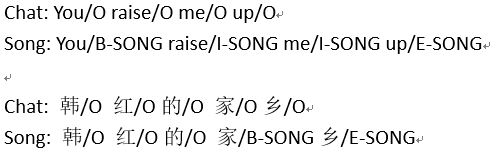
\includegraphics[width=.9\columnwidth]{gazzete_is_needed} % Reduce the figure size so that it is slightly narrower than the column. Don't use precise values for figure width.This setup will avoid overfull boxes. 
\caption{For NER situation in music service, dictionary is necessary to do NER task. Given the certain knowledge, we tend to denote the corresponding words as a song rather than others.}
\label{fig_gazzete}
\end{figure}

\subsection{Contributions}

In summary, we make these contributions:

\begin{itemize}
\item We proposed a new conception: Outer Dictionary Network (ODN), which is used to update the content of dictionary without retraining the model.
\item We proposed a new structure, Tag Embedding LSTM (TE-LSTM), to realize ODN. The networks use the word tag knowledge, rather than the word itself, to improve the performance of NER tasks.
\item Experiment results have shown that, our model gives significant improvements on dictionary depended-on tasks among many state-of-the-art models.
\item We release a new dataset in music service domain, for further scientific research.
\end{itemize}

\section{Related Work}
Success of BERT \cite{bert} and XLNet \cite{xlnet} show that input embedding knowledge is important and useful for many upper NLP tasks. More useful knowledge is there in the input vector, more efficiently the model would work. To a great degree, embedding layer decides the performance. Many useful features have been explored in NER jobs, such as character level message, word level message, position message, handwriting message. Dictionary knowledge is one of them. Especially in some NER task, like music service, dictionary is heavilly depended on to make better performance. 

Most of the recent models use dictionary as word embedding input, or the word's string format, to give the model related message. Lattice LSTM \cite{lattice}  use the dictionary message as additional input to character baseline LSTM, which can give the model more sentence knowledge. Lexicon Rethinking CNN \cite{lrcnn}, incorporate the dictionary knowledge into correlated CNN layer, and then the coflict word tokens could be solved by rethinking. Stanford NER \cite{stner} use the dictionary knowledge as string format feature, matched them in sentences, in CRF model.

However, in some pratical areas, the content of dictionary will change greatly and constantly. In this way, most of the recent model need to be retrained after every abundantly change. To solve this problem, we need to construct a model which can still be used after such change. We then come up with the idea of ODN, and use TE-LSTM to realize this idea. As a result, no more word embedding is needed, and model needs only to be trained once.  What we need is only the word tag knowledge to help the model better understand user's intention.

\section{Outer Dictionary LSTM}




In this chapter, we illustrate the specific method we use to realize the ODN. Our framework is based on Tensorflow \cite{tensor}. We use the character baseline model for Chinese NER task, inspired by the results of Lattice LSTM \cite{lattice} and Lexicon Rething CNN \cite{lrcnn}. For English NER task, we use the word embedding. In order to better understand the model, we make a appointment that: In Chinsese or other hieroglyphics language, character means a single word; and word is a character phrase which has length longer than one. In English or other letter based language, character means a single letter, and a word is a composition of letters; then a phrase is composited of a sequence of words. For Chinese NER jobs, only character embedding will we use, and no more word embedding is needed, for we hold the following views towards these jobs:

\begin{itemize}
\item Common characters in hieroglyphics language, can be exhaustive, especially for Chinese, because there are no more than 100, 000 characters in simplified Chinese. Therefore, no OOV problem will there be when we use character embedding in Chinese NER task. For English NER task, common used words can approximately treat as limited.
\item Words in hieroglyphics language, will be uncountable, because there are still many new words or pharases are still created every day. Thus, OOV error can not be avoided in these case.
\end{itemize}

Based on that, only character embedding will be use in Chinese NER jobs, to avoid OOV problem. We denote a sentence as a sequence of many characters: $s = (c_1, c_2, ..., c_n)$.

\subsection{Character Based LSTM}

We use character embedding lookup table $e_c$ to turn character id to vector:

\begin{equation}
a_i = e_c(c_i) \label{char_embedding}
\end{equation}

Usually a dropout layer is connected with the embedding output, which is proved useful in NER jobs \cite{mahovy}. After that, bi-directional LSTM (Bi-LSTM), the most common structure used in NER tasks, is applied to learn the character relationship within the sentence. We use the hidden vector for LSTM output, that is, for input: $x = (a_1, a_2, ..., a_n) $,  we get output: $h = (h_1, h_2, ..., h_n)$, where $h_i$ is the concatenation of forward ($\overrightarrow{h_i}$) and backward ($\overleftarrow{h_i}$) LSTM hidden vector:

\begin{equation}
h_i = [\overrightarrow{h_i};\overleftarrow{h_i}] \label{lstm_out}
\end{equation}

\subsection{Tag Embedding Model}

As cases show in Figure \ref{fig_gazzete}, we need to use dictionary for certain NER tasks. However, the constant variation of dictionary may lead to constant retraining problem. Therefore, we may not use the specific word in each dictionary, instead, only the outer knowledge will be used, which is the main principle in ODN. Here, we implement our ODN through Tag Embedding (TE), which uses the tag embedding as the outer knowledge for dictionary. Cause we use LSTM structure to utilize tag embedding, we call our network TE-LSTM.

Specifically, we do this by two step: 

a)  Match sentence with the word in dictionary using certain outer model method.

b)  Turn match result into embedding vector, used as the input of LSTM.



\textbf{Match Policy}. In this part, we need to match all the words in given dictionary occured in current sentence. We impletement this by using Aho-Corasick Automation Algorithm \cite{acalg}. In summary, we build a KMP \cite{kmp} + Trie Tree \cite{trietree} algorithm to accomplish this task. In methematical, given sentence $s = (c_1, c_2, ..., c_n) $, and a dictionary $d_i$, which is composed of word set $D_i=\{w_1, w_2, ..., w_V\}$. We denote the result of match policy as:

\begin{equation}
r_{d_i, j} = [ (f_1, b_1), (f_2 , b_2), ..., (f_k, b_k) ] \label{match_result}
\end{equation}



Here, $f_i$ and $b_i$ denote the front and back position of each match word in original sentence. Let $W_{f_i,b_i}$ represent the substring of sentence $s$ with the rank $[f_i, b_i]$, then each $(f_i, b_i)$ tuple forms a word in $D_i$. Parameter $k$ means the total number of such word matched in $d_i$, which is uncertain. Cause there will be conflict intervals after AC algorithm is performed, we need to select the meaningful intervals, the footnote $j$ thus means that there will be many valid interval arrays. To format the input, we make the following policy to select our valid interval arrays:


\begin{figure}[t]
\centering
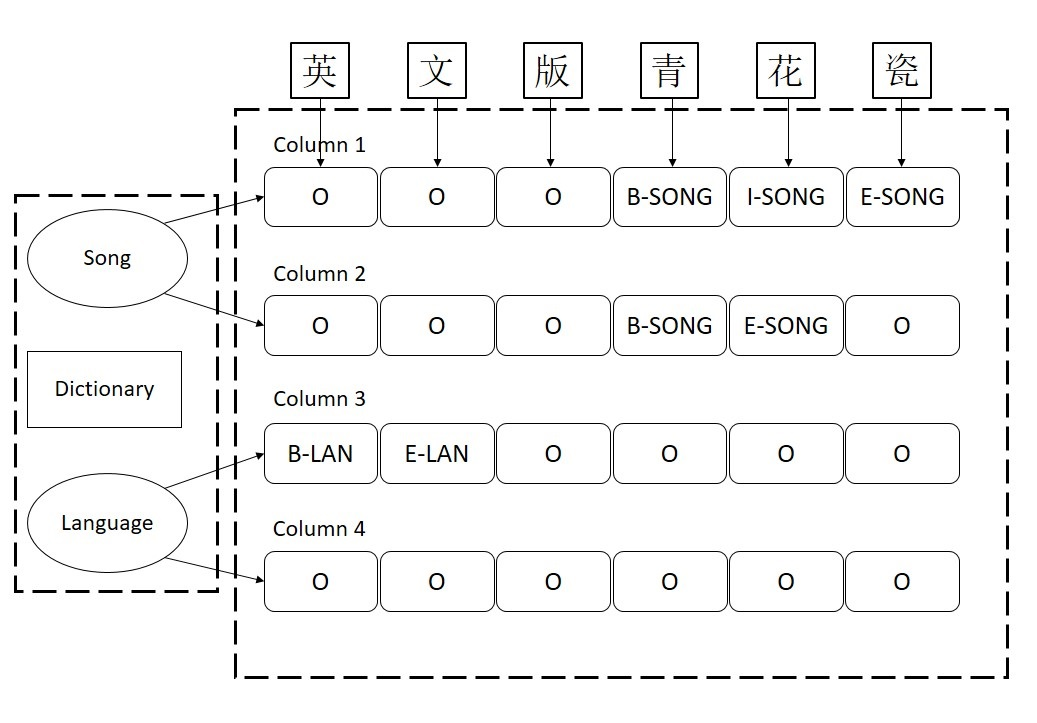
\includegraphics[width=0.9\columnwidth]{tag_scheme} % Reduce the figure size so that it is slightly narrower than the column. Don't use precise values for figure width.This setup will avoid overfull boxes. 
\caption{Illustration for tag embedding scheme. For dictionary `song', there are two possible entities, the longer one is put in the first place (column 1). For dictionary `language', only one possible entity will be matched, however in this case, since we set the tag blank number to 2, we should add one more padding blank to fill the position, which is showed as column 4. }
\label{tag_scheme}
\end{figure}

\begin{itemize}
\item We choose certain number of valid interval arrays, which is called \textbf{tag blank number}, denoted as $w$. If there is not enough candidate interval arrays, the padding interval array will be use to fill out the left position. 
\item We choose the interval arrays which cover the most characters in sentence (words for English), and have no conflict intervals inside itself. And the more characters the interval array has, the prior it will be in embedding position.
\end{itemize}



\textbf{Tag Embedding Scheme}. After match policy is fullfilled, we need to turn that result into vector so that it can be understood by model. Cause the result of match policy is denoted as position, we can simply use it to get a new sequence form from original sentence. With dictionary $d_i$ and a matched word position rank range $[f_i, b_i]$, we then apply tag scheme for that range: turn the match word in that range to corresponding tag as shown in Figure \ref{tag_scheme}, the unmatched part is turned to tag \textbf{O}.

Here, we choose \textbf{IOBES} scheme for it is proved better than IOB1 and IOB2 tag scheme in result by previous works \cite{char-fea1,mahovy}. Yet we need to emphasis that: the tag of dictionary here need not to be the same with the result tag species. As an illustration, to extract \textbf{organization} entity, we can use dictionary \textbf{organization suffix} to supply the suffix knowledge.

As related before, we choose \textbf{tag blank number}, $w$, of valid interval arrays and perform the tag scheme. We do the tag scheme in this way cause we think the position is important for model to understand, which here means to fix the certain tag result in appointed position. Of course, $w$ could be variable for different dictionaries, but that needs a bit more effort and seems low performance increase.

With the tag embedding sequence produced, denoting each tag sequence as: $s_t = (t_1, t_2, ..., t_n)$, we turn the result to vector using: 

\begin{equation}
g_i = e_t(t_i) \label{tag_embedding}
\end{equation}

where $e_t$ is the tag embedding lookup table. We use random uniform generated vector to setup this lookup table. Then the character embedding output $a_i$ and tag embeddding output $g_i$ is concatenated together:
\begin{equation}
x_i = (a_i;g_i) \label{concat}
\end{equation}
Same to Character Based LSTM, a dropout layer is used on the concatenated result. Then the input is fed into the Bi-LSTM layer.  

\begin{table}[t]
\caption{Statistics of Sogou MusicNER dataset.}\smallskip
\centering
\resizebox{.8\columnwidth}{!}{
\smallskip\begin{tabular}{l|c|c|c}
\hline
Count & Sentences & Tokens & Entities\\
\hline
Train & 7,177 & 55,613 & 8,585 \\
Dev & 897 & 6,858 & 1,057 \\
Test & 897 & 6,775 & 1,047 \\
\hline
\end{tabular}
}
\label{table1}
\end{table}



\subsection{Loss and Training}

CRF layer is applied on the top, same with many previous works \cite{nlp,char-fea1,mahovy,comb,lattice,lrcnn}. Denote $y_j$ as a possible label sequence for sentence $s_i$ and $Y$ as the total set of all possible $y_j$, then the probability of $y_j$ is:

\begin{equation}
p(y_j | s_i) = softmax(\sum_i{W_{c_i} * h_i} + B_{c_i})_j
\label{crf_probability}
\end{equation}

$W_{c_i}$, $B_{c_i}$ is respectively the emission matrix and transformation matrix correlate to $h_i$, and $j$ is the rank for $y_j$ in all possible label sequence set $Y$.  While training, we take the $L_2$ regularization for all parameters into account together with CRF loss. With batch number $N$ and corresponding gold set $(s_i, y_i)$, the final loss can be computed as:

\begin{equation}
L = \sum_{i=1}^{N}{log(p(y_i | s_i))} + \frac{\lambda}{2}{|| \theta ||}^2
\label{crf_probability}
\end{equation}

$\lambda$ is the $L_2$ hyper parameter, and $\theta$ stands for all the training parameters. At decoding step, we use the Viterbi algorithm \cite{viterbi} to decode the result, finding the label sequence with the highest score: 

\begin{equation}
y^* = \mathop{\arg\max}_{y_i \in Y}{p(y_i | s_i)}
\label{crf_decode}
\end{equation}




\section{Experiments}

\subsection{Settings}

Here display the experiment settings within our work.

\textbf{Dataset}. For Chinese NER tasks in social domain, we first explore the dataset, \textbf{Weibo NER} \cite{peng15,hesun16} and \textbf{ResumeNER} \cite{lattice}, also used in Lattice LSTM \cite{lattice} and Lexicon Rethinking CNN \cite{lrcnn}. In music domain, We use the dataset obtained from China Conference on Knowledge Graph and Semantic Computing (CCKS) 2018 \cite{ccks}. Cause we could only get the training dataset,  we split that file into three part with portion 8:1:1 as train set, dev set and test set. Call this dataset as \textbf{CCKS} dataset. Another music domain dataset is annotated by ourselves, and the tags are richer than CCKS. The statistics information of this dataset is listed in Table \ref{table1}. We call it \textbf{Sogou MusicNER} dataset. For English NER task, we report the result on \textbf{CoNLL 2003} shared task \cite{conll}.

\textbf{Data Preprocessing}. In our paper, all input file is turned to a certain format, which we call standard NER format. For example, ``\textbf{Peter/B-PER Blackburn/E-PER}'' is turned to string as \textbf{\{``text'': ``Peter Blackburn'', ``slot'': [0, 15, ``PER'''\}}. The numbers stand for the start position and end position in the original sentence. We do it this way since we can get the original input sentence without spliting sentence, and turn it into all other tag scheme (mainly IOB1, IOB2, IOBES) conveniently. Furthermore, we can easily statistics the sentence number and entity number in this format. On training, we turn the standard NER format into the tag scheme we appointed in hyperparameter file. In this way, take the CoNLL 2003 dataset as example, it will first be transformed into standard format, and then turned to IOBES tag scheme when training. In truth, this transformation doesn't change the content of dataset at all, but make it easier to process different format of dataset, and allow us to get the original input sentence to match the dictionary.

\textbf{Character Embedding}. In order to compare with Lattice LSTM (Zhang and Yang 2018) and Lexicon Rethinking CNN (Gui et al. 2019), we use the word vector provided in their papers (these two paper use the same character embedding and word embedding). There are character embedding and word embedding, we use the latter one as character embedding in our model, for we treat English word as a character in Chinese NER task, not a set of single English letters. For English NER task, we use Stanford's public available GloVe word embedding \cite{glove}, 100-dimensional, same with the BLSTM-CNNs-CRF \cite{mahovy}.

\textbf{Tag Embedding}. As related before, we use uniform random policy to generate tag embedding lookup table. Given all tag number $l_t$ and tag embedding size $d_t$ as hyper parameter, we generate a matrix with shape $(l_t, d_t)$ for tag embedding lookup table.

\textbf{Dictionary Knowledge}. For Lattice LSTM and Lexicon Rethinking CNN, they use the same word embedding file to explore dictionary knowledge. For Stanford NER \cite{stner} model, which we will use in our experiment for comparison, we use different dictionaries for different dataset. And the same dictionaries will be use in TE-LSTM, the mehod we proposed. That is to say, for the same dataset, the dictionaries used in Stanford NER and TE-LSTM keep the same. We make up the dictionaries according to the follow principles:

\begin{itemize}
\item For exhaustive tag, we list all the items of that tag, extracted from \textbf{Knowledge Graph}, as a dictionary. For example, entity \textbf{Country} and \textbf{Project}.
\item For tag which is limited but updated constantly, we list the current items of that tag, collected from \textbf{Knowledge Graph}, as a dictionary. For example, entity \textbf{Singer} and \textbf{Song}.
\item For tag that is unlimited but has common prefix or suffix, we list all the common prefix or suffix as a dictionary. For example, entity \textbf{Organization} usually has a common suffix, such as: inc., company, league.
\item For tag which is unlimited and seems no rule inside, we don't use dictionary for it.
\item We setup the dictionaries mainly through \textbf{Knowledge Graph} we build, some of the dictionaries are enriched with the dataset.
\end{itemize}

Comply with these principles, the dictionaries can be built and maintained for pratical use.

\textbf{Handcrafted Features}. Handcrafted features is only used in Stanford NER model. The specific features used in our experiment can be seen in our code. We also explored CRFsuite tools \cite{CRFsuite} to test handcrafted features, but we finally choose Stanford NER for its convenience.


\subsection{Compared Models}

For comparison, we impletement these models below:

\textbf{Lattice LSTM}. The author of Lattice LSTM \cite{lattice} has generously provided his code on website. We directly use his code and settings, and run it on experiment dataset. We denote it as La-LSTM.

\textbf{Lexicon Rethinking CNN}. Same with Lattice LSTM, we use the code obtained from the author's website \cite{lrcnn} and run it on our dataset. We denote it as LR-CNN.

\textbf{Character LSTM}. We impletement the character-level LSTM as the based model, no any other properties (like bichar, softword, position etc.) used. Denoted as C-LSTM.

\textbf{Stanford NER model}. Stanford NER tool \cite{stner} is used in our work to do comparision, for it is convenient to add handcrafted features and use dictionary (called gazette in its term) into model, which can be compared to our ODN intuitively. For short, denote it as ST-NER. 

\textbf{Tag Embedding LSTM}. This is the model which we proposed in this paper. The character embedding is the same with C-LSTM, and the dictionary used is the same with ST-NER model for comparison. We denote it as TE-LSTM.

\subsection{Hyper-parameters and Strategies}

\begin{table}[t]
\caption{Hyperparameters}\smallskip
\centering
\resizebox{.95\columnwidth}{!}{
\smallskip\begin{tabular}{c|c|c|c}
\hline
Hyper-parameters & Value & Hyper-parameters & Value  \\
\hline
char embeddding size & 50 & tag embedding size & 10 \\
lstm state size & 200          & tag blank number & [1,3] \\
lstm layers & 1                   & batch size & [1,10] \\
dropout rate & (0.0, 0.5]     & initial learning rate & [0.01,0.03] \\
decay rate & 0.05              & gradient clipping & 5.0 \\
momentum & 0.9               & L2 $\lambda$ & 1e-8 \\
\hline
\end{tabular}
}
\label{table2}
\end{table}

Shown in Table \ref{table2}, we choose the hyper-parameters referring to BLSTM-CNNs-CRF structure \cite{mahovy}. Main training strategies we used are list as follow:

\begin{itemize}
\item \textbf{Fine-tuning}.We apply fine-tuning on all the embedding vector, which is proved useful by previous works \cite{nlp,peng15,mahovy}. 
\item \textbf{Dropout}. We choose the dropout rate between 0.0 and 0.5, for different dataset to get the best result.
\item \textbf{SGD policy}. We use stochastic gradient descent (SGD) policy to train model, with momentum set to 0.9.
\end{itemize}

\subsection{Main Results}

\begin{table}[t]
\caption{Main Results on Weibo NER.}\smallskip
\centering
\resizebox{.8\columnwidth}{!}{
\smallskip\begin{tabular}{l|ccc}
\hline
Model & NE & NM & Overall  \\
\hline
La-LSTM  & 53.04\% & 62.25\% &  58.79\%  \\
LR-CNN  & \textbf{57.14}\% & 66.67\% & 59.92\%  \\
\hline
C-LSTM & 51.03\% &47.58\% & 49.25\%  \\
ST-NER & 46.69\% & 57.32\% & 52.04\% \\
TE-LSTM & 48.78\% & \textbf{71.31}\% & \textbf{60.10}\%  \\
\hline
\end{tabular}
}
\label{table_weibo}
\end{table}

\begin{table}[t]
\caption{Main Results on ResumeNER.}\smallskip
\centering
\resizebox{.8\columnwidth}{!}{
\smallskip\begin{tabular}{l|ccc}
\hline
Model & Precision & Recall & F1  \\
\hline
La-LSTM  & 94.81\% & 94.11\% &  94.46\%  \\
LR-CNN  & \textbf{95.37}\% & 94.84\% & 95.11\% \\
\hline
C-LSTM & 94.31\% & 94.27\% & 94.29\%  \\
ST-NER & 94.15\% & 93.74\% & 93.94\%  \\
TE-LSTM & 95.32\% & \textbf{95.15}\% & \textbf{95.24}\%  \\
\hline
\end{tabular}
}
\label{table_resume}
\end{table}

\begin{table}[t]
\caption{Main Results on CCKS.}\smallskip
\centering
\resizebox{.8\columnwidth}{!}{
\smallskip\begin{tabular}{l|ccc}
\hline
Model & Precision & Recall & F1  \\
\hline
La-LSTM  & 87.34\% & 75.03\% &  80.72\%  \\
LR-CNN  & 88.17\% & 76.98\% & 82.20\%  \\
\hline
C-LSTM & 75.66\% & 71.12\% & 73.32\%  \\
ST-NER & \textbf{91.00\%} & 76.15\% & 82.92\%  \\
TE-LSTM & 84.28\% & \textbf{84.51\%} & \textbf{84.40\%}  \\
\hline
\end{tabular}
}
\label{table_ccks}
\end{table}

\begin{table}[t]
\caption{Main Results on Sogou MusicNER.}\smallskip
\centering
\resizebox{.8\columnwidth}{!}{
\smallskip\begin{tabular}{l|ccc}
\hline
Model & Precision & Recall & F1  \\
\hline
La-LSTM   & 86.24\% & 84.43\% & 85.33\% \\
LR-CNN   & 85.99\% & 85.00\% & 85.49\% \\
\hline
C-LSTM  & 84.11\% & 82.50\% & 83.30\% \\
ST-NER  & 88.00\% & 85.48\% & 86.72\% \\
TE-LSTM  & \textbf{93.09\%} & \textbf{92.82\%} & \textbf{92.96\%} \\
\hline
\end{tabular}
}
\label{table_sogou}
\end{table}

\begin{table}[t]
\caption{Main Results on CoNLL 2003.}\smallskip
\centering
\resizebox{.8\columnwidth}{!}{
\smallskip\begin{tabular}{l|ccc}
\hline
Model & Precision & Recall & F1  \\
\hline
Ma and Hovy, 2016   & 91.35\% & 91.06\% & 91.21\% \\
Yang et al. 2018 & --- & --- & 91.35\% \\
Devlin et al. 2018   & --- & --- & 92.80\% \\
\hline
C-LSTM  & 87.32\% & 85.25\% & 86.27\% \\
ST-NER  & 86.02\% & 84.63\% & 85.32\% \\
TE-LSTM  & \textbf{96.63\%} & \textbf{96.67\%} & \textbf{96.65\%} \\
\hline
\end{tabular}
}
\label{table_conll}
\end{table}



Compared to previous work, we report the best result of our experiment here.

\textbf{Weibo NER Dataset}. As comparison to previous works, shown in Table \ref{table_weibo}, we report the F1-score for named entities (NE), nominal  entities (NM) and overall entities. The dictionaries we use here are the set of \textbf{GPE\_NAM}, \textbf{ORG\_NOM}, \textbf{PER\_NOM}, \textbf{LOC\_NOM} and \textbf{Chinese Last Name}. We report the highest F1-score on this dataset, higher than LatticeLSTM and LR-CNN.

\textbf{ResumeNER Dataset}. Dictionary \textbf{Title Suffix}, \textbf{Organization Suffix}, \textbf{Project} and \textbf{China Peoples} is used here on ST-NER and TE-LSTM. Results on this dataset also support the efficiency of ODN.

\textbf{CCKS / Sogou MusicNER Dataset}. Table \ref{table_ccks} and \ref{table_sogou} show the result of music domain dataset. The mainly dictionaries used here is \textbf{Singer} and \textbf{Song}. Results show that our model report the best result on both dataset on F1-score. With dictionary information given, we can see that ST-NER shows better performance than La-LSTM and LR-CNN. That, to some extent, cause by the lack of music domain knowledge in La-LSTM and LR-CNN. Compared to ST-NER, our model gives \textbf{1.48\%} percent promotion of F1-score on \textbf{CCKS} dataset, and \textbf{6.24\%} percent promotion on \textbf{MusicNER} dataset. The results prove that TE-LSTM is effective to utilize the knowledge of dictionary, though, without specially making word embedding vector for each word.

\textbf{CoNLL Dataset}. On this dataset, we list some of the effective model results reported by previous works. And we use dictionary \textbf{English Last Name}, \textbf{Location}, \textbf{Organization}, \textbf{MISC}. We make a suppose here that we can get all the real entities of location, organization and miscellaneous in English. With this prerequisite, we could see significant improvement on this dataset, 3.85\% percent over BERT \cite{bert} on F1-score, shown in Table \ref{table_conll}. Though the result is amazing, \textbf{we need to emphasis that, it is hard and burdensome to collect all the entities in these dictionaries in reality}. For simplicity, we use the set of entities extracted from the dataset instead. So the result is only used to show that, ODN is powerful in using dictionary knowledge, but the way to collect dictionaries on this dataset is impratical, conflict with the principles we build dictionaries before.

\subsection{Analysis}



As a further summarization for experiment results, we make the following conclusions:

\textbf{No OOV problem}. We don't need to consider OOV problem for the networks in ODN, for we only use character-based networks, and we only collect the dictionary which is exhaustive among all time or a certain time range. Furthermore, only the tag knowledge is used in ODN, not the specific word.

\textbf{Dictionary is important}. By comparing the results between C-LSTM and TE-LSTM, we would find great improvement after dictionary knowledge is given to model.

\textbf{Powerful in using dictionary knowledge}. Though without any handcrafted features, our model, TE-LSTM, performs better than ST-NER, with the same dictionary knowledge given.

\textbf{Helpful to Improve Recall}. All the experiment results on different dataset get the highest recall score, proving that ODN is a powerful tool on recall.

\textbf{More efficient when dictionary is more necessary}. By comparing the results on CCKS and Sogou MusicNER dataset to La-LSTM and LR-CNN, our model give significant improvement on these dataset, mainly because dictionary is necessary in music domain and, both La-LSTM and LR-CNN lack the knowledge of that. Results on CoNLL can also prove this view if the necessary dictionary can be built. On other datasets, the improvement is not so significant.

\textbf{Conflict Solving}. Though given dictionary knowledge, there exist many conflict items, labeled with different tag, to challenge the model. For example,  ``\textbf{French Open}'', The word ``\textbf{French}'' will be given both the \textbf{S-MISC} tag and \textbf{B-ORG} tag here. TE-LSTM can solve these conflict cases well by using the dictionary knowledge together with the character embedding knowledge, as we could see in Table \ref{table_conll}, 

\textbf{Without Retraining}. We show it here that TE-LSTM need not to retrain the model when dictionary is greatly changed. The cost of retraining a model is changed to be the cost of maintaining the dictionaries, which is more convenient and can be understood and modified by human. 

Here, we use entity \textbf{Song}, in CCKS dataset, as example. Figure \ref{fig3} shows the difference after adding corresponding words into dictionary \textbf{Song}, the model can then recognize these entities with the new given knowledge. Figure \ref {fig4} shows the change after deleting redundant words in dictionary, the model will ignore these words after that operation. But there are also cases which will not change or partly change after deleting the words, shown in Figure \ref{fig5},  these cases exist because there exist certain word phrases to discriminate the word as a song,  or because part of the word is still in the dictionary. Retraining the model will make no sense on solving this problem usually.

\begin{figure}[t]
\centering
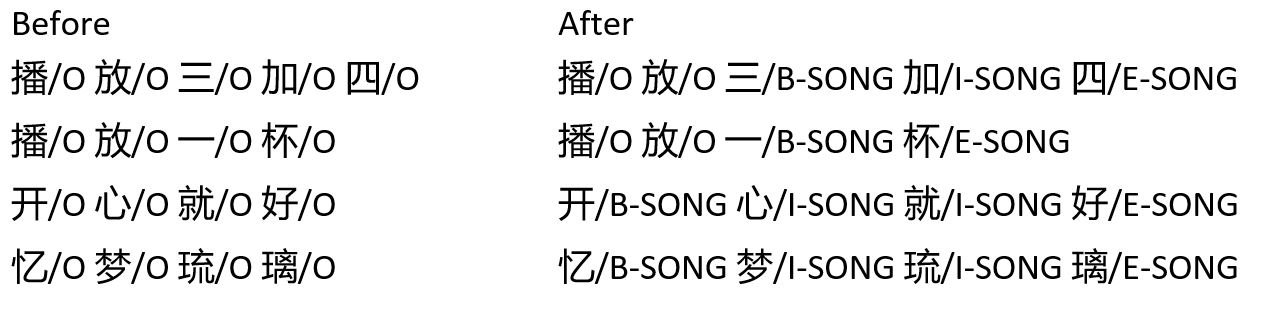
\includegraphics[width=0.9\columnwidth]{change_after_adding_song} % Reduce the figure size so that it is slightly narrower than the column. Don't use precise values for figure width.This setup will avoid overfull boxes. 
\caption{In music service, after adding corresponding words into song dictionary, the new entities can be recognized by the model without retraining.}
\label{fig3}
\end{figure}

\begin{figure}[t]
\centering
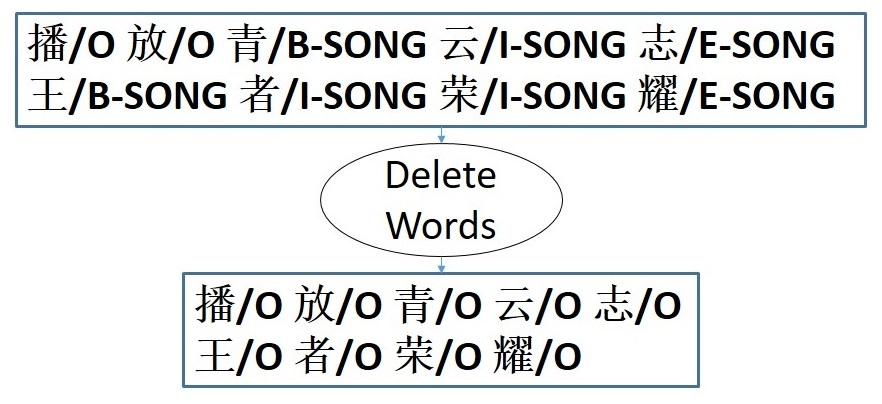
\includegraphics[width=0.85\columnwidth]{change_after_delete_song} % Reduce the figure size so that it is slightly narrower than the column. Don't use precise values for figure width.This setup will avoid overfull boxes. 
\caption{In music service, after delete corresponding words in dictionary, the corresponding entities can be ignored by the model without retraining.}
\label{fig4}
\end{figure}

\begin{figure}[t]
\centering
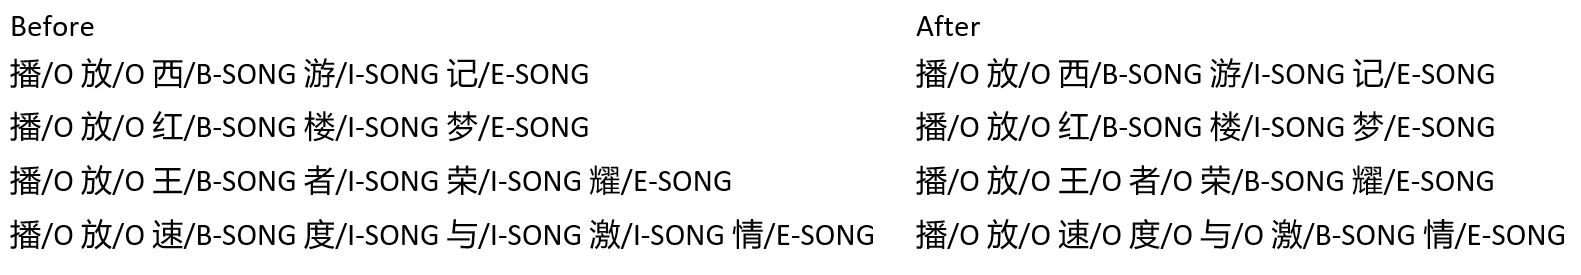
\includegraphics[width=0.85\columnwidth]{no_change_after_delete_song} % Reduce the figure size so that it is slightly narrower than the column. Don't use precise values for figure width.This setup will avoid overfull boxes. 
\caption{In music service, after delete corresponding words in dictionary, some of the the result will not change. Retraining will no help on these cases.}
\label{fig5}
\end{figure}

\section{Conclusion}

We proposed a new model to better explore the knowledge of dictionary without making embedding vector for each word, which helps us need not to retrain a model after the content of dictionary is greatly changed. And the results show that our model reach higher performance on dictionary-depended task, which certificated that our model is a powerful structure to utilize the knowledge of dictionary. And with ODN, the cost of training a new model is replaced by protecting the dictionaries, which is more understandable to human beings.

We have several directions to move ahead. For the structure itself, ODN can also be simply implemented using other structure, like the Lattice LSTM structure or CNNs structure, which also, is a powerful way to use dictionary knowledge. To solve the problem that, entity is still be recognized by the model after it is deleted from dictionary, we can construct a negative dictionary that contains list of words which we don't want it to be recognized. Furthermore, we can investigate networks that could search the needed knowledge from website or knowledge graph by itself, which is more useful and promising in pratical.

\section{ Acknowledgments }

Especially grateful to Can Cui (Chengdu, Operational Platform Department, Sogou Inc.) for cooperation on the Sogou MusicNER dataset, to Jindou Wu (Hangzhou, AI Research Department, Sogou Inc.) for advice on data processing of CCKS 2018 music dataset and handcrafted features on StanfordNER tools.

\bibliographystyle{aaai}
\bibliography{OD-LSTM_GE}

\end{document}
